\begin{figure}[h]
\centering
\begin{minipage}{0.48\textwidth}
\centering
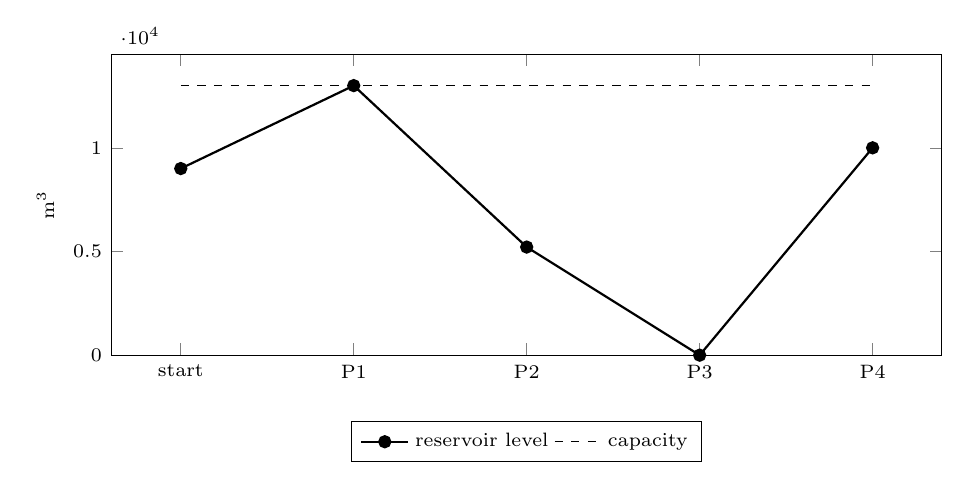
\begin{tikzpicture}
\begin{axis}[
  width=\linewidth, height=5.4cm,
  symbolic x coords={start,P1,P2,P3,P4}, xtick=data,
  ymin=0, ymax=14500, ylabel={m$^3$},
  legend style={font=\scriptsize, at={(0.5,-0.22)}, anchor=north, legend columns=-1},
  tick label style={font=\scriptsize}, label style={font=\scriptsize}]
\addplot[thick, mark=*] coordinates {(start,9000) (P1,13000) (P2,5214) (P3,0) (P4,10000)};
\addplot[dashed] coordinates {(start,13000) (P4,13000)};
\legend{reservoir level, capacity}
\end{axis}
\end{tikzpicture}

\small (a) Reservoir level at the end of each period
\end{minipage}\hfill
\begin{minipage}{0.48\textwidth}
\centering
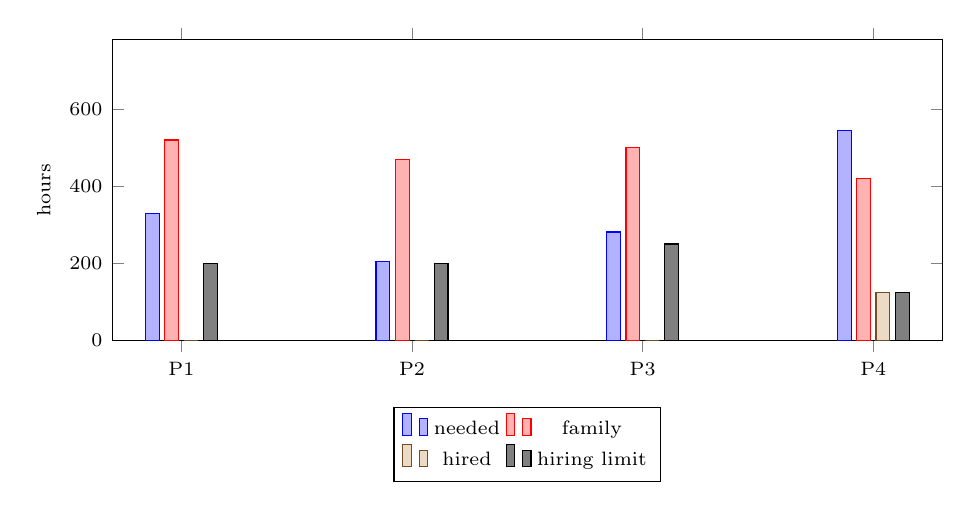
\begin{tikzpicture}
\begin{axis}[
  width=\linewidth, height=5.4cm,
  ybar, bar width=5pt,
  symbolic x coords={P1,P2,P3,P4}, xtick=data,
  ymin=0, ymax=780, ylabel={hours},
  legend style={font=\scriptsize, at={(0.5,-0.22)}, anchor=north, legend columns=2},
  tick label style={font=\scriptsize}, label style={font=\scriptsize}]
\addplot coordinates {(P1,328.3) (P2,204.4) (P3,281.2) (P4,545.0)};
\addplot coordinates {(P1,520) (P2,470) (P3,500) (P4,420)};
\addplot coordinates {(P1,0) (P2,0) (P3,0) (P4,125)};
\addplot coordinates {(P1,200) (P2,200) (P3,250) (P4,125)};
\legend{needed, family, hired, hiring limit}
\end{axis}
\end{tikzpicture}

\small (b) Work needed, family hours and hired hours
\end{minipage}
\caption{How the optimal plan uses the reservoir and the hired labour.}
\label{fig:water-labour}
\end{figure}
